%!TEX root=../GaugeCNNTheory.tex


\subsubsection*{Global rotation and scale equivariance on $\fakebold{\Euc}_{\boldsymbol{2}} \fakebold{\backslash} \bm{\{0\}}$ via log-polar coordinates}
\label{sec:polar_Euc2_logpolar}

\begin{figure}
    \centering
    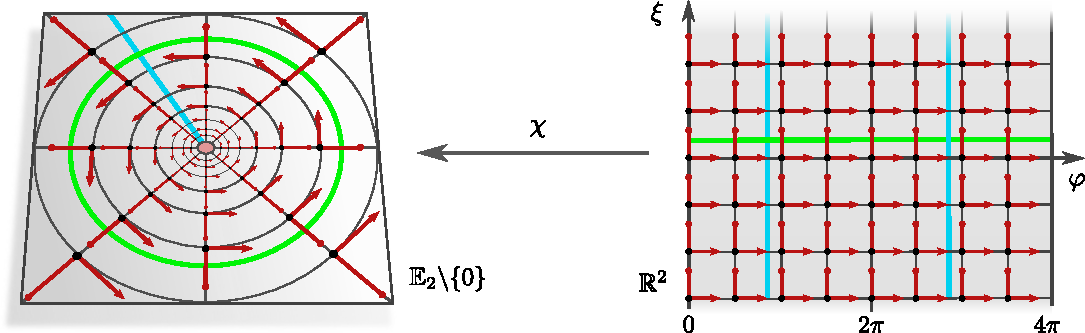
\includegraphics[width=.94\textwidth]{figures/G_structure_R2_no_origin_logpolar_coords.pdf}
    \vspace*{2ex}
    \caption{\small
        Log-polar coordinates 
        $\chi: \R^2 \to \R^2 \backslash \{0\} :\, (\varphi,\xi) \mapsto \big( e^{\xi}\cos(\varphi) ,\, e^{\xi}\sin(\varphi) \big)$
        map angles $\varphi \in \R$ and log-radii $\xi = \log\lVert p\rVert \in \R$ to points $p$ in $\R^2 \backslash \{0\}$.
        After choosing Cartesian coordinates of $\Euc_2 \backslash \{0\} \cong \R^2 \backslash \{0\}$, this yields a coordinatization of $\Euc_2 \backslash \{0\}$ by $\R^2$.
        The log-polar coordinates imply an $\{e\}$-structure on $\Euc_2 \backslash \{0\}$, consisting of reference frames
        $\big[ \frac{\partial}{\partial \varphi} ,\, \frac{\partial}{\partial \xi} \big]$ that are aligned with the coordinate grid.
        They furthermore induce a Riemannian metric, which differs from the usual Euclidean metric and relative to which the induced frames are orthonormal.
        $\GM$-convolutions on the $\{e\}$-structure correspond to conventional Euclidean convolutions in the coordinates $\R^2$.
        Translations $(\Delta\varphi,\, \Delta\xi) \in \Trans_2$ on $\R^2$ correspond via $\chi$ to rotations and rescalings of $\Euc_2 \backslash \{0\}$, where the rotation angles and rescaling factors are given by $\Delta\varphi$ and $e^{\Delta\xi}$, respectively.
        The translation equivariance of the convolution in coordinates $\R^2$ implies therefore the ${\SO2 \!\times\! \Scale}$-equivariance of the $\GM$-convolution on $\Euc_2 \backslash \{0\}$.
        This result is in agreement with the isometry equivariance of the $\GM$-convolution since the transformations in $\IsomGM = {\SO2 \!\times\! \Scale}$ are isometries relative to the induced metric.
        \citet{esteves2017polar} implement such $\GM$-convolutions in terms of conventional convolutions on $\R^2$.
     }
    \label{fig:G_structure_R2_no_origin_logpolar}
\end{figure}


By making the rotation invariant $G$-structures from the last section additionally scale invariant, the corresponding $\GM$-convolutions become equivariant w.r.t. the direct product group ${\SO2 \!\times\! \Scale}$.
Such $G$-structures are induced by \emph{log-polar coordinates}, shown in Fig.~\ref{fig:G_structure_R2_no_origin_logpolar}, which allow for a convenient implementation of the $\GM$-convolution in terms of conventional Euclidean convolutions on the coordinate representation $\R^2$.
The translation equivariance of convolutions on $\R^2$ corresponds then to the ${\SO2 \!\times\! \Scale}$-equivariance on $\Euc_2 \backslash \{0\}$.
For clarity, we start by describing the model in terms of log-polar coordinates as proposed by \citet{esteves2017polar}.%
\footnote{
    The idea to implement rotation invariant correlations via log-polar transforms appeared already in the 80's~\cite{saito1983scale,casasent1987real}.
}
Subsequently, we investigate how this model and its properties are explained in our framework.


Log-polar coordinates of the punctured Euclidean vector space $\R^2 \backslash \{0\}$ are defined in terms of the smooth surjection
\begin{align}
    \chi:\, \R^2 \to \R^2 \backslash \{0\} \,,\ \ 
    (\varphi, \xi) \mapsto \big( e^\xi \cos(\varphi) ,\, e^\xi \sin(\varphi) \big) \,,
\end{align}
which assigns points $p = \chi(\varphi,\xi)$ in $\R^2 \backslash \{0\}$ to a given polar angle $\varphi \in \R$ and log-radius ${\xi = \log\lVert p\rVert \in \R}$.
This map is $2\pi$-periodic in the angular coordinate (note the repetition of the blue stripe on the r.h.s. of Fig.~\ref{fig:G_structure_R2_no_origin_logpolar}) and is therefore in particular non-injective.
A restriction to $[0,2\pi) \times \R$ would be bijective and continuous, however, not homeomorphic -- this will require us below to consider at least two charts to cover the punctured plane.
Cartesian coordinates identify $\R^2 \backslash \{0\}$ with $\Euc_2 \backslash \{0\}$, and therefore allow to assign log-polar coordinates to the latter.
As different (right-handed) Cartesian coordinate systems that are centered in the origin of $\Euc_2 \backslash \{0\}$ differ only by rotations, the assignment of log-polar coordinates is ambiguous by a shift in the angular component.


Given a feature map $f: \R^2 \backslash \{0\} \to \R^c$ (an $\eM$-associated feature field, as clarified below), \citet{esteves2017polar} consider its pullback $\tilde{f} := f \circ \chi \ : \R^2 \to \R^c$ via log-polar coordinates, defined by the commutativity of the following diagram:
\begin{equation}
\begin{tikzcd}[row sep=2.5em, column sep=5.em]
    \R^2
        \arrow[r, "\chi"]
        \arrow[rr, rounded corners, to path={ 
                |- node[below, pos=.75]{\small$\tilde{f}$} ([yshift=-2.5ex, xshift=0ex]\tikztotarget.south)
                -- ([xshift=0ex]\tikztotarget.south)
                }]
    & \R^2 \backslash \{0\}
        \arrow[r, "f"]
    & \R^c
\end{tikzcd}
\end{equation}
A rotation and scaling equivariant group convolution of the feature field~$f$ on $\R^2 \backslash \{0\}$ is then defined by
1)~pulling it via $\chi$ back to coordinates $\R^2$
2)~applying a conventional Euclidean convolution there and
3)~mapping the result back to $\R^2 \backslash \{0\}$.
This procedure is well defined since $\chi$ is smooth, such that smooth feature maps (feature fields) $f$ result in smooth and periodic pullbacks $\tilde{f}$.
Since convolutions are position independent, their output feature map will still be periodic and smooth, and corresponds therefore uniquely to a smooth feature map on $\R^2 \backslash \{0\}$.%
\footnote{
    To see this, note that $\chi$ is a quotient map (since its angular part is a quotient map $\R \to S^1 \cong \R/2\pi\Z$).
    For continuous (instead of smooth) feature maps the statement follows from the universal property of quotient spaces; see e.g.
    \href{https://en.wikipedia.org/wiki/Quotient_space_(topology)\#Properties}{\underline{Wikipedia}}.
    As the smoothness of a function is defined as its continuous differentiability, the universal property can be applied recursively to show that the statement holds for smooth feature maps as well.
}

The rotation and scaling equivariance of the implied group convolution on $\R^2 \backslash \{0\}$ follows from the translation equivariance of the coordinate function~$\chi$.%
\footnote{
    That this is possible relies on the fact that there is a group homomorphism
    $\Trans_2 \to \SO2 \!\times\! \Scale,\ (\Delta\varphi,\, \Delta\xi) \mapsto (R_{\Delta\varphi},\, e^{\Delta\xi})$,
    defined by the group isomorphism $\exp: \Trans_1 \to \Scale$ on the second factor and the group homomorphism (quotient map) $R: \Trans_1 \to \SO2 \cong \Trans_1 / 2\pi\Z$ on the second factor, where $R_{\Delta\varphi}$
    \mbox{denotes the rotation matrix by an angle of $\Delta\varphi$.}
}
Let $(\varphi, \xi)$ be any coordinates in $\R^2$ and let $(\Delta\varphi, \Delta\xi)$ be any translation in $\Trans_2$.
The point of $\R^2 \backslash \{0\}$ that corresponds to translated coordinates ${(\varphi \!+\! \Delta\varphi} ,\, {\xi \!+\! \Delta\xi)}$ relates then to the point corresponding to non-translated coordinates $(\varphi, \xi)$ via a scaling by the factor $e^{\Delta\xi}$ and rotation by the angle $\Delta\varphi$:
\begin{align}\label{eq:log_polar_translation_equivariance}
    \chi \big( \varphi+\Delta\varphi ,\, \xi+\Delta\xi \big)
    \ &=\ e^{\xi+\Delta\xi} \begin{pmatrix} \cos(\varphi+\Delta\varphi) \\ \sin(\varphi+\Delta\varphi) \end{pmatrix} \notag \\
    \ &=\ e^{\Delta\xi}
        \begin{pmatrix} \cos(\Delta\varphi)\mkern-8mu & -\sin(\Delta\varphi) \\ \sin(\Delta\varphi)\mkern-8mu & \phantom{-} \cos(\Delta\varphi) \end{pmatrix}
        e^\xi \begin{pmatrix} \cos(\varphi) \\ \sin(\varphi) \end{pmatrix} \notag \\
    \ &=\ e^{\Delta\xi}
        \begin{pmatrix} \cos(\Delta\varphi)\mkern-8mu & -\sin(\Delta\varphi) \\ \sin(\Delta\varphi)\mkern-8mu & \phantom{-} \cos(\Delta\varphi) \end{pmatrix}
        \chi(\varphi,\, \xi) \notag \\
    \ &=:\ (\Delta\varphi,\, \Delta\xi) \,\rhd\, \chi(\varphi,\, \xi)
\end{align}
In terms of a diagram, this means that
\begin{equation}
\begin{tikzcd}[row sep=3.5em, column sep=7.em]
    \R^2
        \arrow[r, "(\Delta\varphi {,}\, \Delta\xi) +"]
        \arrow[d, "\chi\,"']
    & \R^2
        \arrow[d, "\,\chi"]
    \\
    \R^2 \backslash \{0\}
        \arrow[r, "(\Delta\varphi {,}\, \Delta\xi) \rhd"']
    & \R^2 \backslash \{0\}
\end{tikzcd}
\end{equation}
commutes for arbitrary translations.
Together with the translation equivariance of conventional convolutions on $\R^2$, this implies that rotated and scaled input feature maps on $\R^2 \backslash \{0\}$ will lead to rotated and scaled output feature maps on $\R^2 \backslash \{0\}$, i.e. the ${\SO2 \!\times\! \Scale}$-equivariance of the convolution on $\R^2 \backslash \{0\}$.
More details on this viewpoint are found in~\cite{esteves2017polar} and~\cite{blatt1994canonical}.


We will now revisit this convolution operation and its properties from the viewpoint of coordinate free $\GM$-convolutions.
To do so, we consider an atlas of charts that are consistent with the log-polar coordinates, and discuss the induced $\{e\}$-structure, gauges, Riemannian metric, geodesics and parallel transport that it implies.
The claimed ${\SO2 \!\times\! \Scale}$-equivariance follows immediately from the $\IsomeM$-equivariance of $\GM$-convolutions.
For notational convenience, we will again identify $\Euc_2 \backslash \{0\}$ via some choice of Cartesian coordinates with $\R^2 \backslash \{0\}$.

As the restriction $\tilde{\chi}: [0,2\pi) \times \R \to \R^2 \backslash \{0\}$ of the log-polar coordinates $\chi$ to non-redundant angles is bijective and continuous, one might be tempted to take its inverse as a coordinate chart.
This is, however, not possible, since $\tilde{\chi}$ is not a homeomorphism, as required for charts.
Instead, we consider an atlas consisting of two charts that are defined in terms of restrictions of $\chi$ and that cover $\R^2 \backslash \{0\}$.
One particular choice is to define chart codomains as open sets $V^A = (0,2\pi) \times \R$ and $V^B = (-\epsilon,\epsilon) \times \R$ for some $0< \epsilon <\pi$ and, for $X=A,B$, define charts on $U^X = \chi(V^X)$ as $x^X := \big( \chi\big|_{V^X} \big)^{-1} : U^X \to V^X$.
Intuitively, this atlas achieves the same as the naive attempt to define charts as the inverse $\tilde{\chi}$.
The important difference is, however, that the charts are diffeomorphic, which is necessary to assure the smoothness of all operations.


As usual, these charts induce local frame fields and bundle trivializations on $U^A$ and $U^B$, respectively.
It is easy to see that the transition maps $g_p^{BA} = \frac{\partial x^B}{\partial x^A} |_{x^A(p)}$ on $U^A \cap U^B$ are trivial, which implies that the union of the frame fields defines a smooth $\{e\}$-structure $\eM$ on $\R^2 \backslash \{0\}$.
These coordinate bases, which are in the literature often denoted as $\big[ \frac{\partial}{\partial \varphi} ,\, \frac{\partial}{\partial \xi} \big]$, are shown in Fig.~\ref{fig:G_structure_R2_no_origin_logpolar} (left).
Our calculation in Eq.~\eqref{eq:log_polar_translation_equivariance} above implies that the induced $\{e\}$-structure is ${\SO2 \!\times\! \Scale}$-invariant.


The charts induce furthermore a Riemannian metric, which differs from the usual Euclidean metric on $\R^2 \backslash \{0\}$.
It is defined as the pullback of the Euclidean metric $\langle \cdot,\cdot \rangle_{\R^2}$ in the charts' codomains, and is therefore pointwise given by
\begin{align}
    \eta_p(v,w) \,:=\, \big\langle \hat{d}x^X_p(v) \,,\, \hat{d}x^X_p(w) \big\rangle_{\R^2} \,,
\end{align}
where $v,w \in \TpM$ and $X$ denotes either chart with $p\in U^X$.
The chart induced $\{e\}$-structure consists by construction of \emph{frames that are orthonormal w.r.t. this chart induced metric}, even though these \emph{frames grow with the radius when measured relative to the standard Euclidean metric}.
The Levi-Civita connection of the induced metric differs from the usual Euclidean connection and implies therefore alternative geodesics and parallel transporters.
As the metric is pulled back via the charts, the geodesics correspond to straight lines in the charts' codomains -- an example are the coordinate lines on $\R^2 \backslash \{0\}$ in Fig.~\ref{fig:G_structure_R2_no_origin_logpolar}.
The parallel transport corresponds to the usual transport in the charts' codomains as well, which implies that it keeps transported vectors in a fixed angle to the coordinate lines on $\R^2 \backslash \{0\}$; cf. footnote~\ref{footnote:punctured_Euclidean_transport}.
Note that this is the same transport as already discussed above in the models corresponding to Figs.~\ref{fig:G_structures_R2_no_origin}, where it was \emph{not} the transport corresponding to the Levi-Civita connection since these models assumed the standard metric on $\R^2 \backslash \{0\}$ instead of the chart induced metric.


The $\{e\}$-structure preserving isometries $\IsomeM \cong {\SO2 \!\times\! \Scale}$ \emph{relative to the chart induced metric} are given by rotations and rescaling of the $\{e\}$-structure \emph{relative to the usual Euclidean metric}.
Theorem~\ref{thm:isom_equiv_GM_conv} implies the ${\SO2 \!\times\! \Scale}$-equivariance of the corresponding $\GM$-convolution -- which recovers the statement made by \citet{esteves2017polar} in our theory.
As stated above, the fact that the metric is induced via the charts means that all operations reduce to the usual Euclidean operations when being expressed in the chart.
The $\GM$-convolution is therefore best implemented via a conventional convolution on the chart, as proposed by \citet{esteves2017polar}.


Note that the ${\SO2 \!\times\! \Scale}$-equivariance of the $\GM$-convolution is easily extended to ${\O2 \!\times\! \Scale}$-equivariance, which includes reflections.
This is implemented by performing a reflection equivariant convolution in the chart, which corresponds to the $\Flip$-structure shown in Fig.~\ref{fig:G_structure_R2_3}.
On $\R^2 \backslash \{0\}$, this implies a $\Flip$-structure that looks similar to that in Fig.~\ref{fig:G_structure_R2_no_origin_O2} above, with the difference that the $\Flip$-structure is additionally invariant under a global rescaling.
